\documentclass[10pt]{beamer}
\usepackage{multicol}
\usepackage[english]{babel}
\usepackage{blindtext}
\usepackage{lipsum}
\usepackage{amsmath}
\usepackage{dsfont}
\usepackage{lmodern}
\usepackage{listings}
\usepackage{xcolor}
\RequirePackage{atbegshi}
\usepackage{scalefnt}

\hypersetup{pdfpagemode=FullScreen}
\usetheme{Warsaw}

\usepackage{tikz}
\usetikzlibrary{shadows,patterns,shapes}
% The logic for Hanoi, we record the discs at every pole
% as a comma separated list ending with a '.'; i.e. the
% starting list for 4 discs would be 1,2,3,4,.
\newcount\ndiscs
\def\initpoles#1{
    \def\disclist{}
    \foreach \n in {1,...,#1} {
        \xdef\disclist{\disclist\n,}
    }
    \expandafter\xdef\csname pole 1\endcsname{\disclist.}
    \expandafter\gdef\csname pole 2\endcsname{.}
    \expandafter\gdef\csname pole 3\endcsname{.}
}

% Delimited macro; #1 is everything up to the first ',' and
% #2 everything after it.
\def\head#1,#2.{#1}
\def\tail#1,#2.{#2}

% This macro updates the disc lists, its arguments are the name
% names of the macro's corresponding to the poles, for example
% 'pole 1' and 'pole 3'.
\def\movedisc#1#2{
    \edef\lista{\csname #1\endcsname}
    \edef\listb{\csname #2\endcsname}
    \expandafter\xdef\csname #2\endcsname{\expandafter\head\lista,\listb}
    \expandafter\xdef\csname #1\endcsname{\expandafter\tail\lista.}
}

% Updates the lists and then draws a new frame.
\def\move#1#2{
    \movedisc{pole #1}{pole #2}
    \gdef\fmsg{\node[anchor=north] at (3.8,-.5) {Disco movido de #1 para #2.};}
    \drawpoles
}

% This macro boils down to a well-known recursive solution, as given
% here for example: http://en.wikipedia.org/wiki/Towers_of_Hanoi#Recursive_solution
%
% #1 Pole to move from
% #2 Pole to move to
% #3 Pole to use as scratch
% #4 Number of disks
\def\rhanoi#1#2#3#4{
    \ifnum#4>1
        {\advance#4 by -1 \rhanoi#1#3#2#4}
        \move{#1}{#3}
        {\advance#4 by -1 \rhanoi#2#1#3#4}
    \else
        \move{#1}{#3}
    \fi
}

% Below is the TikZ code to draw the towers:
\tikzset{
    disc/.style={shade, shading=radial, rounded rectangle,minimum height=.5cm,
        inner color=#1!20, outer color=#1!60!gray},
    disc 1/.style={disc=yellow, minimum width=15mm},
    disc 2/.style={disc=orange, minimum width=20mm},
    disc 3/.style={disc=red, minimum width=25mm},
    disc 4/.style={disc=green, minimum width=30mm},
    disc 5/.style={disc=blue, minimum width=35mm},
    disc 6/.style={disc=purple, minimum width=40mm},
}

% Define some colors, I don't like plain green and brown.
\definecolor{darkgreen}{rgb}{0.2,0.55,0}
\definecolor{darkbrown}{rgb}{0.375,0.25,0.125}

\newcommand{\pole}{
  \fill[darkbrown] (-1.6cm, 0) rectangle (1.6cm,0.25cm)
    (-1.25mm,2.5mm) rectangle (1.25mm,4.25cm);
}

% Because the list starts with the topmost disc, we
% use two recursive macro's to invert the drawing process.
\newcount\curlevel

% This macro checks whether the list is empty, if not,
% it calls \rdrawdiscs which removes one element and
% calls this one again.
\def\drawdiscs#1.{
    % If #1 is empty, this expands to \if.. which is true, otherwise
    % we're safe to assume there's at least one element.
    \expandafter\if#1..\else
        \rdrawdiscs#1.
        \advance\curlevel by 1\relax
    \fi
}

\def\rdrawdiscs#1,#2.{
    \drawdiscs#2.
    {\edef\n{\the\curlevel}
        % Draw the actual disk.
        \node[disc #1,yshift={\n*5mm}] {#1};
    }
}

\def\discs#1{
    \curlevel=1
    \expandafter\drawdiscs#1
}

% Draws the whole situation based on the lists.
\def\drawpoles{
    \begin{frame}{\ftitle}
    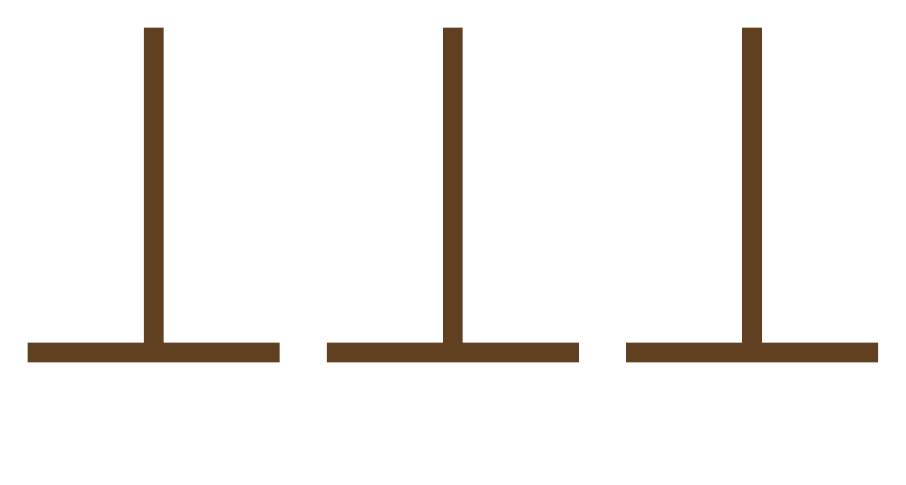
\begin{tikzpicture}
        \foreach \n/\x in {1/0cm,2/3.8cm,3/7.6cm} {
            \begin{scope}[xshift=\x]
                \pole
                \expandafter\discs\csname pole \n\endcsname
            \end{scope}
        }
        % Macro that either contains something like OK or
        % the last move.
        \fmsg
        % We use this to prevent the picture from jumping between
        % frames.
        \useasboundingbox (-1.6cm,-1.2cm) rectangle (9.2cm,4.25cm);
    \end{tikzpicture}
    \end{frame}
}

% Main macro, inits the lists for the current number, sets a title
% for the frame and starts the recursion.
\def\hanoi#1{
    \ndiscs=#1
    \initpoles{#1}
    \ifnum\ndiscs=1
        \xdef\ftitle{Torre de Hanoi -- \the\ndiscs\ Disco}
    \else
        \xdef\ftitle{Torre de Hanoi -- \the\ndiscs\ Discos}
    \fi
    \gdef\fmsg{}
    \center
    \drawpoles
    % Recursion draws a new frame for every step.
    \rhanoi{1}{2}{3}{\ndiscs}
    % Final frame.
    \gdef\fmsg{\node[] at (3.8,2.5) {\Huge\scalefont{2}\color{darkgreen}OK};}
    \drawpoles
}
\definecolor{commentgreen}{RGB}{2,112,10}
\definecolor{eminence}{RGB}{108,48,130}

\newcommand{\duascolunas}[2]{
  \begin{columns}[t]
    \begin{column}{6cm}
      #1
    \end{column}
    \begin{column}{6cm}
      #2
    \end{column}
  \end{columns}
}

\newcommand{\codecpp}[3][0.6]{
  \centering
  \begin{minipage}{#1\textwidth}
    %Referencia: https://ctan.dcc.uchile.cl/macros/latex/contrib/listings/listings.pdf
\lstset{
    language=C++,
    title=#3,
    numbers=left,
    numberstyle=\tiny,
    stepnumber=1,
    numbersep=5pt,
    %framexrightmargin=-4.5cm,
    %framexleftmargin=0mm,
    frame=shadowbox,
    commentstyle=\color{commentgreen},
    keywordstyle=\color{eminence},
    stringstyle=\color{red},
    backgroundcolor=\color{black!3},
    keywordstyle=\color{blue},
    rulesepcolor=\color{black!5},
    basicstyle=\small\ttfamily, % basic font setting
    emph={int,char,double,float,unsigned,void,bool},
    emphstyle={\color{blue}}
    }
  \lstinputlisting{#2}
\end{minipage}}

\usetheme{CambridgeUS}
\title{Recursão}
\subtitle[Recursão]{Algoritmos e Estrutura de Dados II}
\author{Prof. Kennedy Lopes}


\begin{document}

\frame{\titlepage}
\frame{\tableofcontents}
\frame{
  \frametitle{Referência}
  A atual aula tem como principal referência o conteúdo apresentado no livro \textbf{Data Structures and Algorithms in C++} do Adam Drozdek:
  \begin{figure}[h]
    \begin{center}
      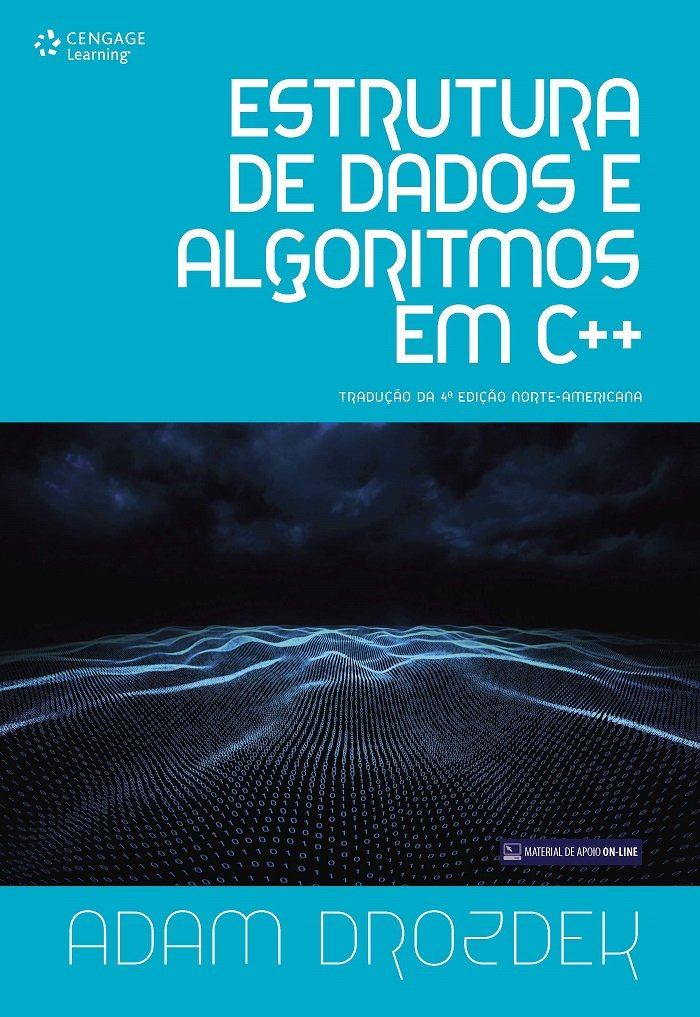
\includegraphics[width=4cm]{fig/img01.jpg}
    \end{center}
  \end{figure}
}

\frame{
  \begin{itemize}
    \item Um procedimento ou função é dito \textbf{recursivo} se este invoca (realiza uma chamada) a si mesmo.
    \item Próprias definições podem ser consideradas recursivas:
          \begin{itemize}
            \item <1- | alert@1> Sistemas de arquivos;
            \item <2- | alert@2> Números naturais;
            \item <3- | alert@3> Dilema ovo-galinha;
            \item <4- | alert@4> Expressões matemáticas;
            \item <5- | alert@5> Lógica de programação.
          \end{itemize}
    \item Conceito está conectado com a relação de recorrência e indução, exemplo:
          $$ a_n = 2*a_n-1; a_0 = 1 \rightarrow a_n = 2^n$$
  \end{itemize}
}

\begin{frame}{Definições}
  \duascolunas{\begin{block}{Caso Base}
      Parte não recursiva, também chamado de âncora, ocorre quando a resposta para o problema é trivial.
    \end{block}
    \vfill
    \begin{block}{Passo indutivo}
      Parteda definição que especifica como cada elemento (solução) é gerado a partir do precedente.
    \end{block}}{
    \begin{figure}[h]
      \begin{center}
        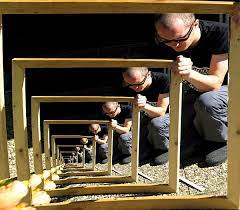
\includegraphics[width=5cm]{fig/droste.jpeg}
        \caption{Efeito Droste}
      \end{center}
    \end{figure}
  }
\end{frame}

\frame{
  \frametitle{Clássico exemplo}
  Cálculo fatorial:
  \begin{equation}
    fat(x)=\begin{cases}
      1,           & \text{if $x=0$}.       \\
      x\ fat(x-1), & \text{caso contrário}.
    \end{cases}
  \end{equation}
  considerando $x \in \mathds{N}$
  \vfill
  \pause

  Exemplo fat(4):

  \begin{columns}[t]
    \begin{column}{6cm}
      \begin{align*}
        \only<2-10> {f(4) & = 4 * fat(3)}             \\
        \only<3-10> {f(4) & = 4 * 3 * fat(2)}         \\
        \only<4-10> {f(4) & = 4 * 3 * 2 * fat(1)}     \\
        \only<5-10> {f(4) & = 4 * 3 * 2 * 1 * fat(0)}
      \end{align*}
    \end{column}
    \begin{column}{6cm}
      \begin{align*}
        \only<6-10> {f(4)  & = 4 * 3 * 2 * (1 * 1)} \\
        \only<7-10> {f(4)  & = 4 * 3 * (2*1)}       \\
        \only<8-10> {f(4)  & = 4 * (3 * 2)}         \\
        \only<9-10> {f(4)  & = (4 * 6)}             \\
        \only<10-10> {f(4) & = 24}
      \end{align*}
    \end{column}
  \end{columns}
}

\begin{frame}[t]
  \frametitle{Cálculo de uma potência}
  Calcula a potência com um expoente inteiro de um número em ponto flutuante.
  \begin{equation*}
    x^n=\begin{cases}
      1,                & \text{se}\ n=0.        \\
      \frac{1}{x^{-n}}, & \text{se}\ n<0.        \\
      x(x^{n-1}),       & \text{caso contrário}.
    \end{cases}
  \end{equation*}

\end{frame}

\begin{frame}
  \frametitle{Exemplo: Números naturais}
  \begin{columns}[t]
    \begin{column}{6cm}
      \begin{itemize}
        \item $0$ pertence aos números naturais.
        \item se $n \in \mathds{N} \rightarrow n+1 \in \mathds{N}$
      \end{itemize}
      \vfill
      Exemplo $2 \in \mathds{N}$?
      \begin{itemize}
        \item <1- | alert@1>Verificar se $2 \in \mathds{N}$
              \begin{itemize}
                \item <2- | alert@2>Verificar se $1 \in \mathds{N}$
                      \begin{itemize}
                        \item<3- | alert@3> Verificar se $0 \in \mathds{N}$
                        \item<4- | alert@4> De fato $0 \in \mathds{N}$
                      \end{itemize}
                \item <5- | alert@5>De fato $1 \in \mathds{N}$
              \end{itemize}
        \item<6- | alert@6> Portanto $2 \in \mathds{N}$
      \end{itemize}
    \end{column}
    \begin{column}{6cm}
      \begin{figure}[h]
        \begin{center}
          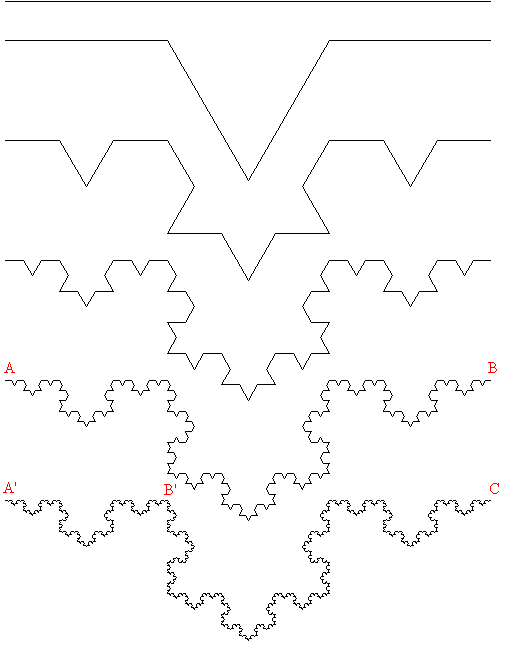
\includegraphics[width=4cm]{fig/img02.png}
        \end{center}
      \end{figure}
    \end{column}
  \end{columns}
\end{frame}

\begin{frame}[t]
  \frametitle{Torre de Hanoi}
  Objetivo: Mover os blocos da base 1 para a base 3, utilizando, caso necessário, a torre central.\footnote{Fonte da animação: https://texample.net/tikz/examples/towers-of-hanoi/}

  Única regra: Um bloco maior não pode ficar em cima de um bloco menor.
  \begin{figure}[h]
    \begin{center}
      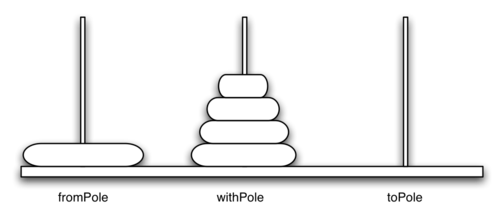
\includegraphics[width=12cm]{./fig/hanoi.png}
    \end{center}
  \end{figure}
\end{frame}

\hanoi{1}
\hanoi{2}
\hanoi{3}

\begin{frame}
  \frametitle{Torre de Hanoi (Algoritmo) - $N>1$}
  MOVER(N, ORIGEM, DESTINO, AUXILIAR)
  \begin{itemize}\itemsep1em 
    \item<2->Passo 1: MOVER(N-1, ORIGEM, AUXILIAR, DESTINO)
    \item<3->Passo 2: MOVER O DISCO DA \textbf{ORIGEM} PARA O \textbf{DESTINO}
    \item<4->Passo 3: MOVER(N-1, AUXILIAR, DESTINO, ORIGEM)
  \end{itemize}

  \vfill
  \begin{figure}[h]
    \begin{center}
      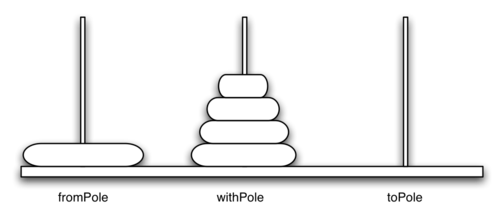
\includegraphics[width=8cm]{./fig/hanoi.png}
    \end{center}
  \end{figure}
  
\end{frame}

\hanoi{4}
% \hanoi{6}


\begin{frame}
  \frametitle{Exemplo: Formação de sequências}
  Funções recursivas são comumente utilizadas para geração de sequências. Exemplo:
  \begin{equation}
    f(n)=\begin{cases}
      1,                         & \text{if $n=0$}.     \\
      f(n-1) + \frac{1}{f(n-1)}, & \text{caso $n > 0$}.
    \end{cases}
  \end{equation}
  \pause
  Sequência gerada:

  $$1, 2, \frac{5}{2}, \frac{29}{10}, \frac{941}{240}, \frac{969581}{272890}, \ldots$$
\end{frame}

\begin{frame}
  \frametitle{Recursão}
  \begin{block}{Consideração}
    Definicões recursivas de sequências tem uma desvantagem: Para determinar o valor de um elemento, e necessário conhecer todos os outros elementos anteriores. Como solução, deve-se encontrar uma expressão iterativa para a resolução sem que seja conhencido os termos anteriores.
  \end{block}
  Exemplo:
  \begin{equation}
    g(n)=\begin{cases}
      1,        & \text{if $n=0$}.     \\
      2*g(n-1), & \text{caso $n > 0$}.
    \end{cases}
  \end{equation}
  \begin{columns}[t]
    \begin{column}{4cm}
      \begin{align*}
        g(0) & = 1 \\
        g(1) & = 2 \\
        g(2) & = 4
      \end{align*}
    \end{column}
    \begin{column}{4cm}
      \begin{align*}
        g(3)   & = 8   \\
        \ldots &       \\
        g(n)   & = 2^n
      \end{align*}
    \end{column}
  \end{columns}
  \vfill
\end{frame}

\begin{frame}
  \frametitle{Recursão}
  Recursão para definições sintáticas de algoritmos:
  \vfill
  \begin{figure}[h]
    \begin{center}
      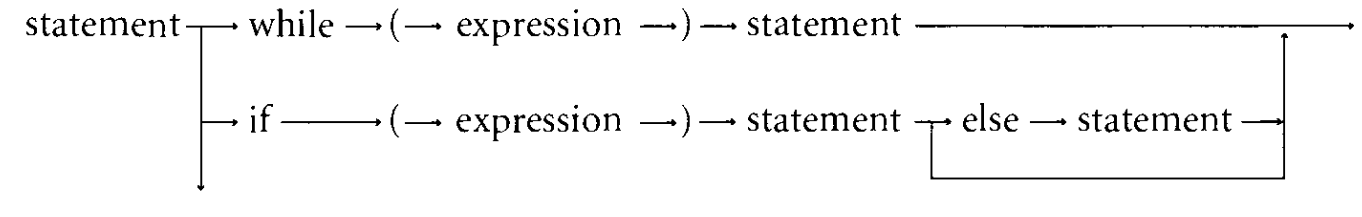
\includegraphics[width=8cm]{fig/img03}
    \end{center}
  \end{figure}
  \vfill
  Ou em BNF: \emph{Backus-Naur Form}
  \vfill
  \begin{figure}[h]
    \begin{center}
      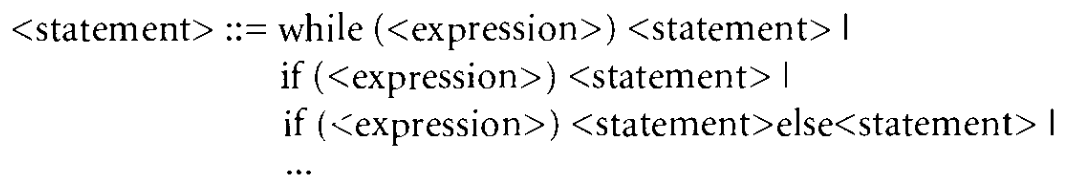
\includegraphics[width=8cm]{fig/img04}
    \end{center}
  \end{figure}

\end{frame}

\begin{frame}
  \frametitle{Chamada de funções e implementação da Recursão}
  \begin{columns}[t]
    \begin{column}{6cm}
      Considere uma função \textbf{main()} que chama \textbf{f1()} que chama\textbf{f2()} que chama \textbf{f3()}:
      \begin{itemize}
        \item Para cada função mais do que apenas o endereço de resposta deve ser armazenado.
        \item Alocação dinâmica é utilizado durante a execução do algoritmo.Cada função com suas próprias variáveis locais.
        \item Faz-se necessário que o contexto de cada função seja \textbf{preservado} antes de cada nova chamada.
      \end{itemize}
    \end{column}
    \begin{column}{6cm}
      \begin{figure}[h]
        \begin{center}
          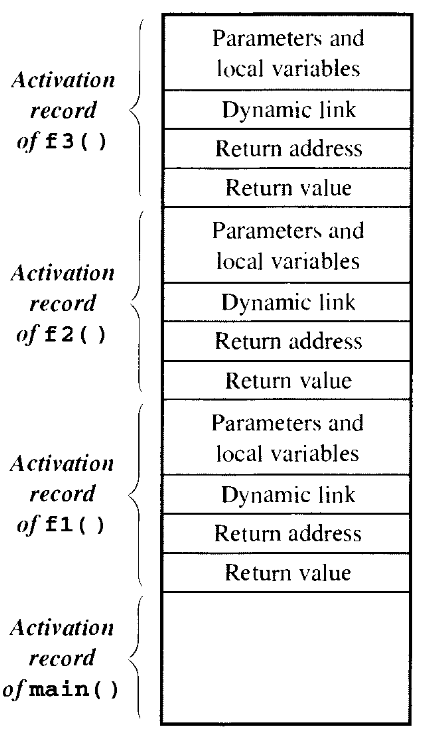
\includegraphics[width=4cm]{fig/img05}
        \end{center}
      \end{figure}
    \end{column}
  \end{columns}
\end{frame}

\begin{frame}
  \frametitle{Chamada de funções e implementação da Recursão}
  \begin{columns}[t]
    \begin{column}{6cm}
      Considere uma função \textbf{main()} que chama \textbf{f1()} que chama\textbf{f2()} que chama \textbf{f3()}:
      \begin{itemize}
        \item Variáveis armazenadas:
              \begin{itemize}
                \item Valores de todos os parâmetros da função;
                \item Variáveis locais que podem ser armazenadas em qualquer outro local;
                \item O endereço de retorno para retomar o controle pelo ativador e o endereço da instrução do ativador;
                \item Um vínculo dinâmico (ponteiro para o registro de ativação do ativador);
                \item O valor retornado par uma função não declarada como \emph{void}.
              \end{itemize}
      \end{itemize}
    \end{column}
    \begin{column}{6cm}
      \begin{figure}[h]
        \begin{center}
          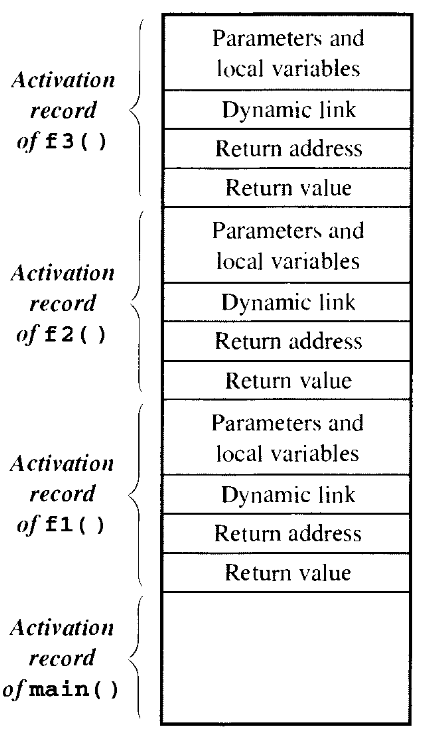
\includegraphics[width=4cm]{fig/img05}
        \end{center}
      \end{figure}
    \end{column}
  \end{columns}
\end{frame}

\section{Anatomia de uma chamada recursiva}
\begin{frame}{Anatomia de uma chamada recursiva}
  Função potência:
  \begin{equation}
    pot(x,n)=\begin{cases}
      1,             & \text{if $n=0$}.     \\
      x*pot(x, n-1), & \text{caso $n > 0$}.
    \end{cases}
  \end{equation}
  \pause
  \codecpp{algoritmos/alg01.c}{Algoritmo Recursivo}
\end{frame}

\section{Recursão de Cauda}
\begin{frame}{Recursão de Cauda}
  \begin{block}{Definição}
    A recursão de cauda é definida pelo uso somente de uma chamada recursiva no final de uma implementação de função. Quando a chamada é recursiva é a \textbf{última operação} a ser realizada dentro da função.
  \end{block}
  \duascolunas{
    \pause
    \codecpp[0.8]{algoritmos/alg02a.c}{Recursão de Cauda}
  }{
    \pause
    \codecpp[0.8]{algoritmos/alg02b.c}{Recursão que não é Cauda}
  }
\end{frame}

\begin{frame}{Recursão de Cauda}
  A recursão de cauda pode ser \textbf{facilmente} substituído por um laço. Convertendo-o a uma função não recursiva.

  \codecpp{algoritmos/alg03.c}{Recursão que não é Cauda}
\end{frame}

\begin{frame}\frametitle{Conversão}
  \center
  \LARGE Conversão de algoritmos recursivos para iterativos
\end{frame}

\begin{frame}
  \duascolunas{
    \codecpp[0.9]{algoritmos/alg04a.c}{Fatorial}
    \codecpp[0.9]{algoritmos/alg04b.c}{Fibonacci}
  }{
    \codecpp[0.9]{algoritmos/alg04c.c}{Somatório}
    \codecpp[0.9]{algoritmos/alg04d.c}{Máximo Divisor Comum}
  }
\end{frame}

\begin{frame}
  \duascolunas{
    \codecpp[0.9]{algoritmos/alg05a.c}{Fatorial Iterativo}
  }{
    \codecpp[0.9]{algoritmos/alg05b.c}{Fibonacci Iterativo}
  }
  \frametitle{Fatorial e Fibonacci Iterativo}
\end{frame}

\section{Recursão que é de Cauda}
\begin{frame}{Recursão que não é de Cauda}
  \duascolunas{
    Algoritmos recursivos que não são de Cauda:
    \begin{itemize}
      \pause \item Qualquer algoritmo recursivo que não tem como última instrução o passo recursivo;
            \pause \item Ocupam mais espaço na execução;
            \pause \item Demandam mais tempo;
            \pause \item O algoritmo tem um tempo de vida menor:
            \begin{itemize}
              \item Por ocupar mais espaço na memória, o programa é finalizado antecipadamente.
              \item Possível erro 1: Memória totalmente ocupada;
              \item Possível erro 2: Programa executado compromente a execução dos sistema.
            \end{itemize}
    \end{itemize}
  }{
    \begin{itemize}
      \pause \item O algoritmo pode ser re-codificado para tornar de cauda. Exemplo:
            \codecpp[0.85]{algoritmos/alg06.c}{Somatório com cauda}
    \end{itemize}
  }
\end{frame}

\section{Recursão indireta}
\begin{frame}{Recursão indireta}
  A chamada recursiva não é executada diretamente:
  \pause
  \begin{align*}
    \textbf{f()} \rightarrow f1() \rightarrow f2() \rightarrow f3() \rightarrow \textbf{f()}
  \end{align*}

  \pause

  As funções intermediárias podem ser re-codificadas como apenas uma única função:

  \begin{align*}
    \textbf{g()} \equiv f1() \rightarrow f2() \rightarrow f3()
  \end{align*}

  Resumindo dessa forma:

  \pause\begin{align*}
    \textbf{f()} \rightarrow g() \rightarrow \textbf{f()}
  \end{align*}

\end{frame}

\begin{frame}
  \frametitle{Recursão indireta}
  \begin{align*}
    \begin{cases}sen(x) &= sen\left(\frac{x}{3}\right) \frac{\left(3-tan^2\left(\frac{x}{3}\right)\right)}{\left(1+tan^2\left(\frac{x}{3}\right)\right)}\\
    tan(x) &= \frac{sen(x)}{cos(x)} \\
    cos(x) &= 1 - sen(\frac{x}{2})
    \end{cases}
  \end{align*}

  Considerando que:

  $$sen(x) \cong x - \frac{x^3}{6}$$
\end{frame}

\section{Recursão Infinita}
\begin{frame}{Recursão Infinita}
  \begin{itemize}
    \item Recursão Infinita provocada por inexistência de caso base.
    \item Pode ser que o caso base seja inalcançável;
    \item O programa irá alcançar o limite da pilha, havendo um \emph{estouro} da memória.
  \end{itemize}
  \pause
  Exemplo:

  \codecpp[0.6]{algoritmos/alg07.c}{Algoritmo com recursão infinita}

\end{frame}

\section*{Recursão excessiva e aninhada}
\begin{frame}
  \frametitle{Recursão excessiva}
  Muito algoritmos recursivos podem ter processamento desnecessário.

  Exemplo: Fibonacci

  \begin{figure}[h]
    \begin{center}
      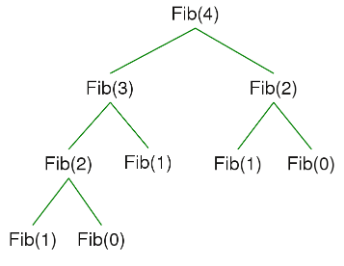
\includegraphics[width=6cm]{fig/fib.png}
      \caption{Árvore de execução da função fibonacci}
    \end{center}
  \end{figure}
\end{frame}

\begin{frame}
  \frametitle{Recursão aninhada}
  Exemplo 1:
  \begin{equation*}
    h(n)=\begin{cases}
      $0$,           & \text{se $n=0$}.     \\
      $n$            & \text{se $n>4$}      \\
      $h(2 + h(n))$, & \text{se $n\leq 4$}.
    \end{cases}
  \end{equation*}

  \pause  Exemplo 2: (Função de Ackerman)
  \begin{equation*}
    A(m,n)=\begin{cases}
      $m+1$,               & \text{se $n=0$}.       \\
      $A(n-1, 1)$          & \text{se $n>4\ e\ m=0$}  \\
      $A(n-1, A(n, m-1))$, & \text{Caso contrário}.
    \end{cases}
  \end{equation*}
\end{frame}

\section{Exercícios}
\begin{frame}{Exercícios}
  \begin{enumerate}
    \item Escreva uma função recursiva para adicionar os primeiros $n$ termos da série:
          $$ 1 + \frac{1}{2} - \frac{1}{3} + \frac{1}{4} - \frac{1}{5} + \ldots$$
    \item Apresente uma versão recursiva da função:
    
    \codecpp[0.6]{algoritmos/alg08.c}{Função cubo}
  \end{enumerate}
\end{frame}

\begin{frame}
  \frametitle{Exercícios}
  \begin{enumerate}
    \setcounter{enumi}{2}
    \item Descreva um algoritmo recursivo para descobrir se uma palavra/expressão é um palíndromo.
    \item Execute à mão o algoritmo fibonacci(5).
    \item Converta o algoritmo Fatorial recursivo para Fatorial recursivo \textbf{com cauda}.
    \item Execute a função de Ackerman à mão (A(4,3)).
    \item Calcule o valor de $sen(80)$ considerando a aproximação apresentada nessa apresentação para valores menores do que $1^o$ e suas definições recursivas.
  \end{enumerate}
  \vfill
\end{frame}

\end{document}